\documentclass[12pt, a4paper]{article}
\usepackage[vmargin=1in,hmargin=1in]{geometry}
\usepackage[pdftex]{graphicx}
\usepackage{amsmath,amssymb}
\usepackage[utf8x]{inputenc}
\usepackage[english]{babel}
\usepackage[pdftex]{graphicx}
\usepackage{ctable}
\usepackage{appendix}
\usepackage{verbatim,listings}
\usepackage{rotating}

\usepackage[lined, boxed]{algorithm2e}

\newcommand{\imsize}{}
\newlength{\widthtmp}
\newcommand{\getWidth}[1]{%
  \settowidth{\widthtmp}{#1}%
  \the\widthtmp%
}
%\providecommand{\abs}[1]{\left\lvert#1\right\rvert}

\usepackage[pdftex,
pdftitle={Antidiffusion techniques to refine the numerical solution of the advection equation. Case study: Smolarkiewicz' iterative approach},
pdfauthor={G. Burger. J. Wolterink},
pdfstartview=FitH
]{hyperref}


\author{Gerhard Burger \and Jelmer Wolterink}
\title{Antidiffusion techniques to refine the numerical solution of the advection equation\\ Case study: Smolarkiewicz' iterative approach}

\newcommand{\abs}[1]{\left\lvert#1\right\rvert}

\begin{document}
\maketitle

\section{Introduction}
The advection equation plays an important role in climate modeling because the advection equation describes a transport mechanism of a substance by a fluid, due to the fluid's motion in a particular direction.
A well known example is the Thermo Haline Circulation (THC).

If the advection equation is solved numerically the space is discretized and this can cause diffusion. Several anti-diffusion techniques are invented to correct for this diffusion. On technique that is still in use today, be it in a generalized form, is the iterative approach developed by Smolarkiewicz in 1983 \cite{smolarki}. This approach is conceptually simple, and straightforward to implement.

In this report we will discuss the implementation of Smolarkiewicz' iterative approach in Fortran. First we will give some general remarks about numerically solving the advection equation and using anti-diffusion techniques, after that we will discuss the actual implementation and finally we will discuss some numerical results and give a short overview of the current developments in anti-diffusion techniques.

\section{Solving the advection equation}
The continuity equation describing the advection of a non-diffusive quantity in a flow field is defined as

\begin{equation}
\frac{\partial \psi}{\partial t} + \text{ div}(V\psi) = 0
\end{equation}

where $\psi(x,y,z,t)$ is the non-diffusive scalar quantity, $V=(u,v,w)$ is the velocity vector and $x,y,z,t$ are the independent variables of space and time.

To solve this equation numerically we need to take into account the following constraints:

\begin{itemize}
\item Solutions should contain no unphysical overshoot or undershoot: positive definite schemes
\item Methods should be volume preserving. No loss of matter
\item The solutions should be local: the solution at any one point should not be influenced by what is going on far away from that point
\item Methods should not introduce new extrema
\end{itemize}

\subsection{Diffusion}
Figure~\ref{fig:dif} provides a nice illustration of what diffusion in 1D is
\begin{figure}[htp]
\renewcommand{\imsize}{0.3\textwidth}
\begin{tabular}{ccc}
{\resizebox{\imsize}{!}{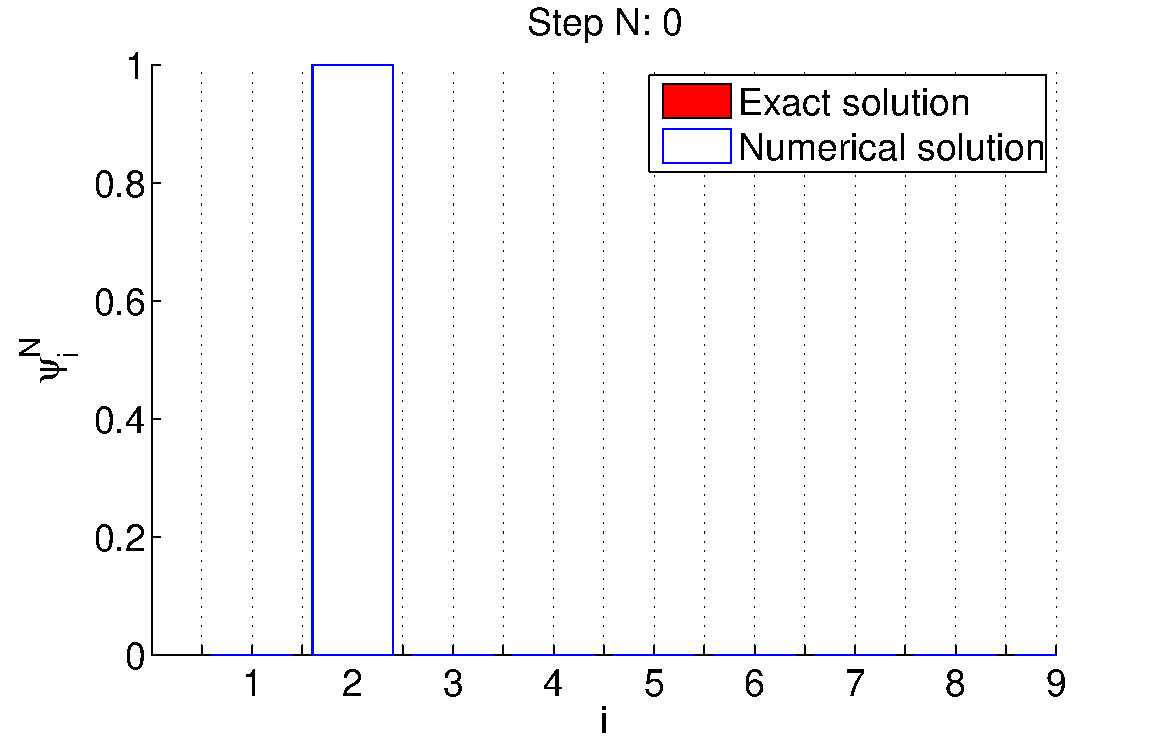
\includegraphics{../presentation/animation/anime0.pdf}}} &
{\resizebox{\imsize}{!}{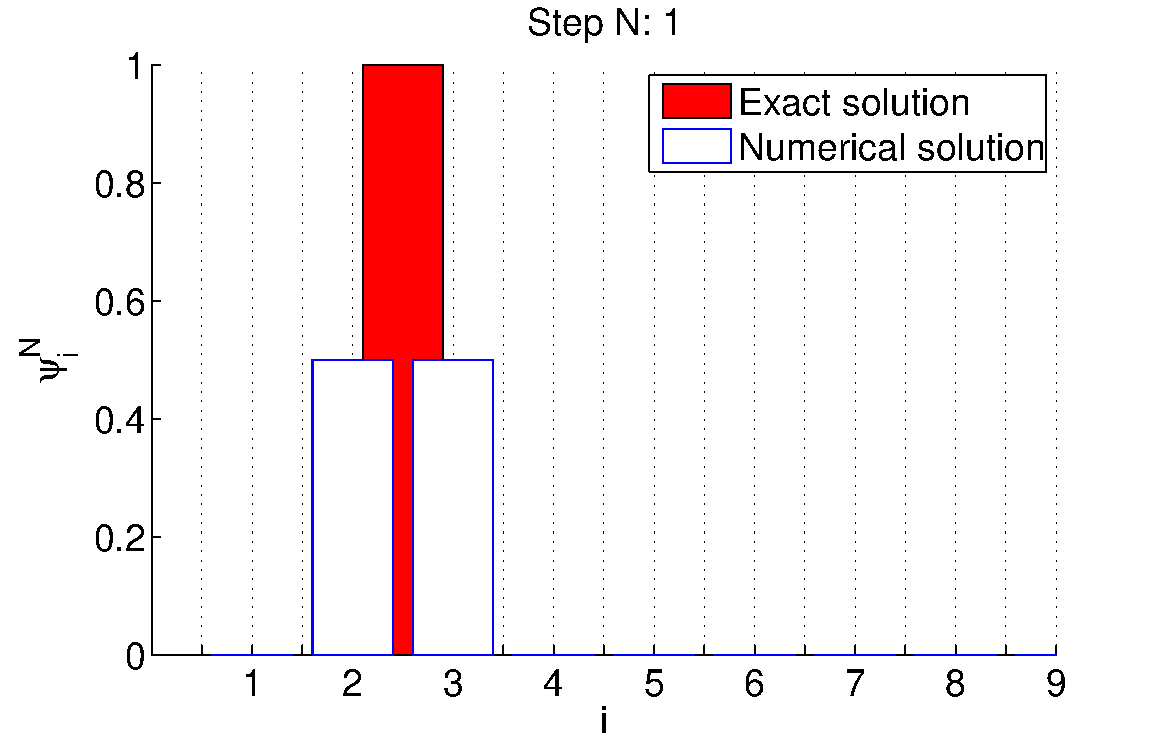
\includegraphics{../presentation/animation/anime1.pdf}}} &
{\resizebox{\imsize}{!}{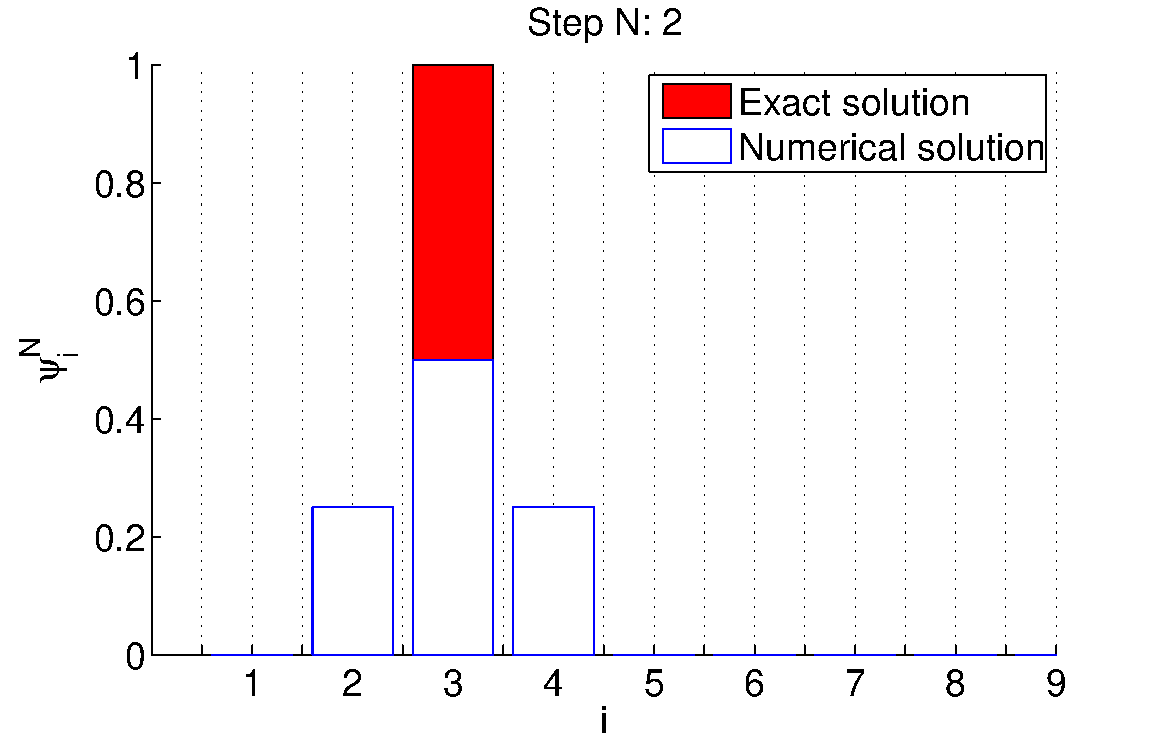
\includegraphics{../presentation/animation/anime2.pdf}}} \\
{\resizebox{\imsize}{!}{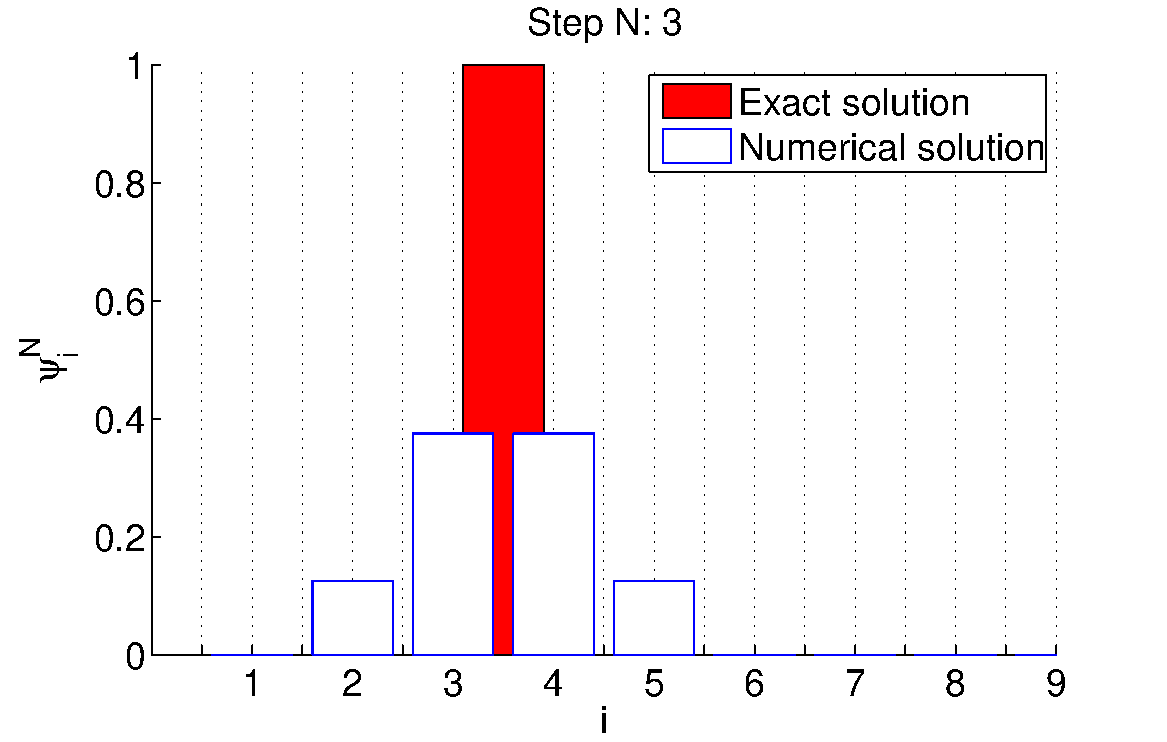
\includegraphics{../presentation/animation/anime3.pdf}}} &
{\resizebox{\imsize}{!}{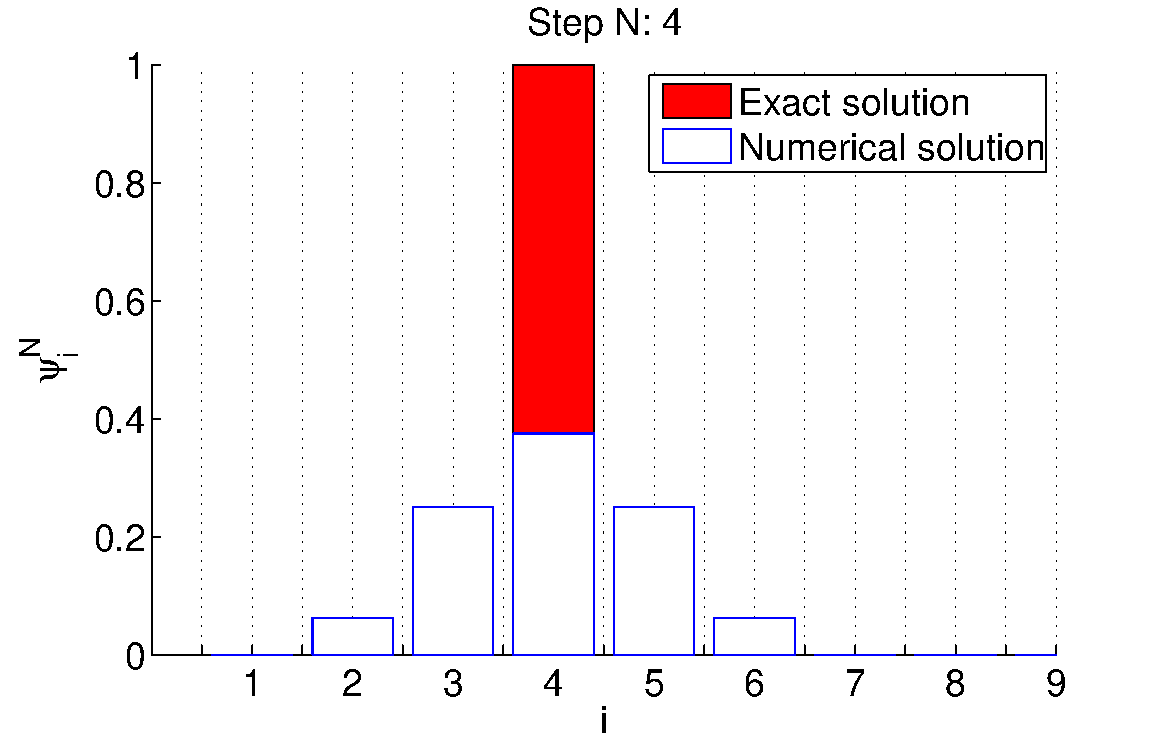
\includegraphics{../presentation/animation/anime4.pdf}}} &
{\resizebox{\imsize}{!}{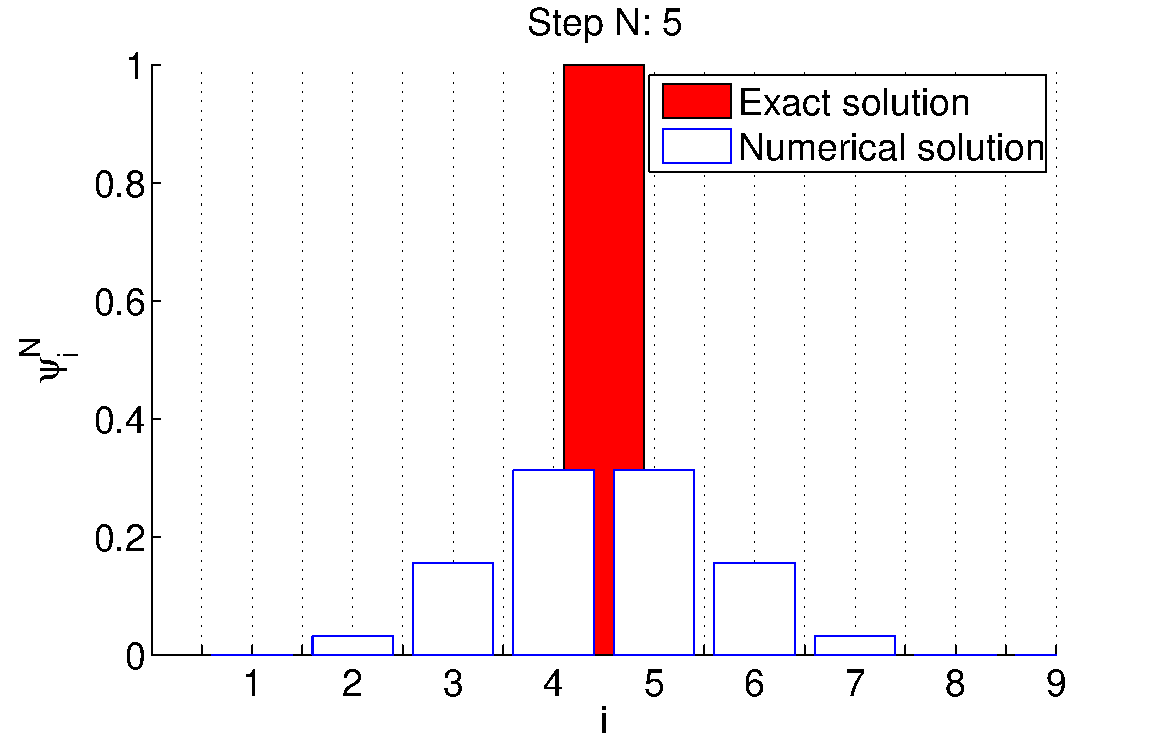
\includegraphics{../presentation/animation/anime5.pdf}}} \\
{\resizebox{\imsize}{!}{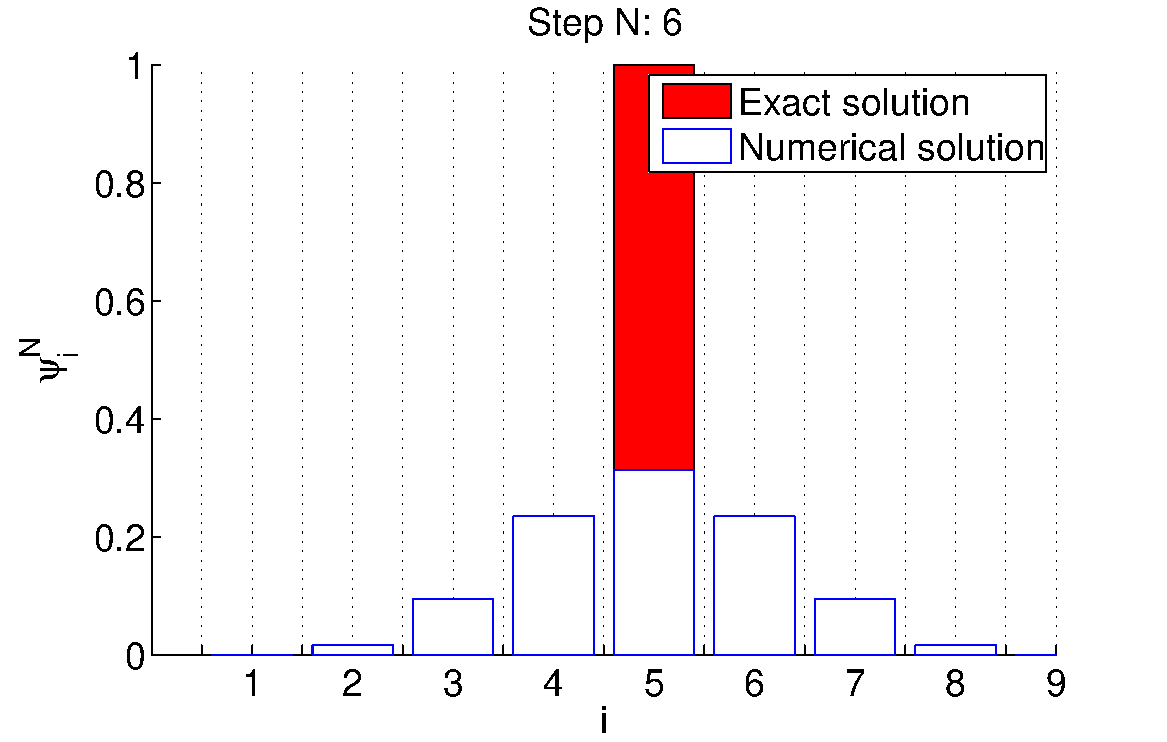
\includegraphics{../presentation/animation/anime6.pdf}}} &
{\resizebox{\imsize}{!}{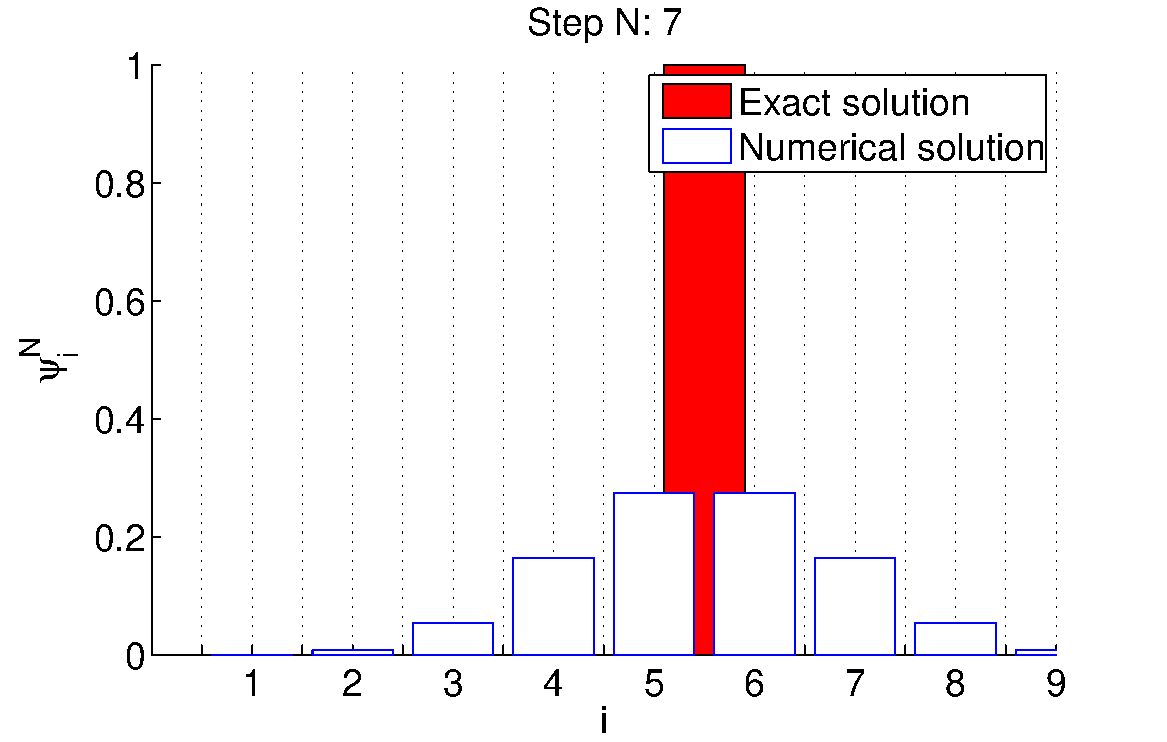
\includegraphics{../presentation/animation/anime7.pdf}}} \\
\end{tabular}
\caption{\label{fig:dif}Example of diffusion when the speed $u=0.5$.}
\end{figure}

In this example the horizontal velocity $u=0.5$ is not integral, so per time step only a portion of the quantity in the gridbox gets moved to the next gridbox. The red bars show the exact solution of the advection equation

\begin{equation}
 u(x,t)=F(x-ut)=F(x-0.5t).
\end{equation}

Clearly this diffusive behavior is undesirable since if your simulation runs for some time, the solution `smears' out and becomes zero everywhere.

\subsection{Anti-diffusion}
To correct for the diffusion in numerical models several techniques were proposed
\section{Case study: Smolarkiewicz}
\subsection{Analyzing the scheme}
\subsection{Implementation}
\subsection{Numerical results}
\section{Current state of research}
\subsection{Possibilities}
\subsection{MPDATA}
\section{Conclusion}



\subsection{One dimensional case}

Upstream advection equation on staggered grid:
\begin{equation}
 \psi_i^{N+1} = \psi_i^N - \Big( F \left( \psi_i^N,\psi_{i+1}^N,u_{i+1/2}^N\right)
-F \left( \psi_{i-1}^N,\psi_{i}^N,u_{i-1/2}^N\right) \Big),
\end{equation}
where
\begin{multline}
F \left( \psi_i^N,\psi_{i+1}^N,u_{i+1/2}^N\right) =\\
\Big( \left( u_{i+1/2}^N + \abs{u_{i+1/2}^N} \right) \psi_i^N
+ \left( u_{i+1/2}^N - \abs{u_{i+1/2}^N} \right) \psi_{i+1}^N \Big)
\frac{\Delta t}{2 \Delta x}.
\end{multline}
This gives
\begin{multline}
\psi_i^{N+1} = \psi_i^N - \frac{\Delta t}{2 \Delta x} \bigg( \Big( \left( u_{i+1/2}^N + \abs{u_{i+1/2}^N} \right) \psi_i^N
+ \left( u_{i+1/2}^N - \abs{u_{i+1/2}^N} \right) \psi_{i+1}^N \Big)
\\
- \Big( \left( u_{i-1/2}^N + \abs{u_{i-1/2}^N} \right) \psi_{i-1}^N
+ \left( u_{i-1/2}^N - \abs{u_{i-1/2}^N} \right) \psi_{i}^N \Big) \bigg).
\end{multline}
Collecting terms gives the method of lines representation
\begin{equation}
\begin{split}
\psi_i^{N+1} &=
\frac{\Delta t}{2 \Delta x} \left( u_{i-1/2}^N + \abs{u_{i-1/2}^N} \right) \psi_{i-1}^N\\
&+ \left(1 - \frac{\Delta t}{2 \Delta x} \left( u_{i+1/2}^N + \abs{u_{i+1/2}^N} - u_{i-1/2}^N + \abs{u_{i-1/2}^N} \right) \right) \psi_i^N\\
&-\frac{\Delta t}{2 \Delta x} \left( u_{i+1/2}^N - \abs{u_{i+1/2}^N} \right) \psi_{i+1}^N\\
\end{split}
\end{equation}

\section*{Two dimensional case}
Upstream advection equation on staggered grid:

\begin{multline}
 \psi_{ij}^{N+1} = \psi_{ij}^N - \Big( F \left( \psi_{ij}^N,\psi_{i+1,j}^N,u_{i+1/2,j}^N\right)
-F \left( \psi_{i-1,j}^N,\psi_{ij}^N,u_{i-1/2,j}^N\right) + \\ F \left( \psi_{ij}^N,\psi_{i,j+1}^N,v_{i,j+1/2}^N\right) -F \left( \psi_{i,j-1}^N,\psi_{ij}^N,v_{i,j-1/2}^N\right) \Big),
\end{multline}

where
\begin{multline}
F \left( \psi_{ij}^N,\psi_{i+1,j}^N,u_{i+1/2,j}^N\right) =\\
\Big( \left( u_{i+1/2,j}^N + \abs{u_{i+1/2,j}^N} \right) \psi_{ij}^N
+ \left( u_{i+1/2,j}^N - \abs{u_{i+1/2,j}^N} \right) \psi_{i+1,j}^N \Big)
\frac{\Delta t}{2 \Delta x}
\end{multline}

and
\begin{multline}
F \left( \psi_{ij}^N,\psi_{i,j+1}^N,v_{i,j+1/2}^N\right) =\\
\Big( \left( v_{i,j+1/2}^N + \abs{v_{i,j+1/2}^N} \right) \psi_{ij}^N
+ \left( v_{i,j+1/2}^N - \abs{v_{i,j+1/2}^N} \right) \psi_{i,j+1}^N \Big)
\frac{\Delta t}{2 \Delta y}.
\end{multline}

This gives

\begin{multline}
 \psi_{ij}^{N+1} = \psi_{ij}^N - \Big( \Big( \left( u_{i+1/2,j}^N + \abs{u_{i+1/2,j}^N} \right) \psi_{ij}^N
+ \left( u_{i+1/2,j}^N - \abs{u_{i+1/2,j}^N} \right) \psi_{i+1,j}^N \Big)
\frac{\Delta t}{2 \Delta x} \\
-\Big( \left( u_{i-1/2,j}^N + \abs{u_{i-1/2,j}^N} \right) \psi_{i-1,j}^N
+ \left( u_{i-1/2,j}^N - \abs{u_{i-1/2,j}^N} \right) \psi_{ij}^N \Big)
\frac{\Delta t}{2 \Delta x} \\
 + \Big( \left( v_{i,j+1/2}^N + \abs{v_{i,j+1/2}^N} \right) \psi_{ij}^N
+ \left( v_{i,j+1/2}^N - \abs{v_{i,j+1/2}^N} \right) \psi_{i,j+1}^N \Big)
\frac{\Delta t}{2 \Delta y} \\
 -\Big( \left( v_{i,j-1/2}^N + \abs{v_{i,j-1/2}^N} \right) \psi_{i,j-1}^N
+ \left( v_{i,j-1/2}^N - \abs{v_{i,j-1/2}^N} \right) \psi_{ij}^N \Big)
\frac{\Delta t}{2 \Delta y} \Big),
\end{multline}

Collecting terms gives the method of lines representation

\begin{equation}
\begin{split}
\psi_{ij}^{N+1} &=
\frac{\Delta t}{2 \Delta y} \left( v_{i,j-1/2}^N + \abs{v_{i,j-1/2}^N} \right) \psi_{i,j-1}^N\\
&+\frac{\Delta t}{2 \Delta x} \left( u_{i-1/2,j}^N + \abs{u_{i-1/2,j}^N} \right) \psi_{i-1,j}^N\\
&+ \Big(1 - u_{i+1/2,j}^N - \abs{u_{i+1/2,j}^N} + u_{i-1/2,j}^N - \abs{u_{i-1/2,j}^N} - v_{i,j+1/2}^N - \abs{v_{i,j+1/2}^N} \\
&+ v_{i,j-1/2}^N - \abs{v_{i,j-1/2}^N} \Big) \psi_i^N\\
&-\frac{\Delta t}{2 \Delta x} \left( u_{i+1/2,j}^N - \abs{u_{i+1/2,j}^N} \right) \psi_{i+1,j}^N\\
&-\frac{\Delta t}{2 \Delta y} \left( v_{i,j+1/2}^N - \abs{v_{i,j+1/2}^N} \right) \psi_{i,j+1}^N\\
\end{split}
\end{equation}


\end{document}
